\chapter{Appendix}\label{ch:appendix}

\section{Machine Configuration}\label{sec:machine-configuration}

The \cref{tab:machine-config} shows the machine configuration used for the experimental setup.

\begin{table}[H]
    \begin{tcolorbox}[arc=0pt,boxrule=0.5pt]
% \sisetup{group-minimum-digits = 4}
        \centering
        \begin{tabular}{ll}
            \toprule
            \textbf{Parameter} & \textbf{Value}
            \\
            \toprule
            Andere Geschwindigkeit für Entlastung & 300 mm/min           \\
            Anzahl Stufen                         & 4                    \\
            Anzahl Zyklen                         & 1                    \\
            Automatische Kraftnullung             & Nein                 \\
            Geschwindigkeit Vorlaufwe             & 100 mm/min           \\
            Geschwindigkeit Zyklus                & 80 mm/min            \\
            Keilspannfaktor                       & 5 bar/kN             \\
            LE-Geschwindigkeit                    & 100 mm/min           \\
            \hdashline
            Maschinendaten                        & 1454MO WN:805754     \\
            Traversenwegaufnehmer                 & WN:805754            \\
            Kraftsensor                           & ID:0 WN:820243 20 kN \\
            \hdashline
            Material                              & Stahl                \\
            Prüfart                               & Druck                \\
            Prüfgeschwindigkeit                   & 5 mm/min             \\
            Prüfnorm                              & DIN 178              \\
            Vorkraft                              & 1 N                  \\
            Vorkraft-Geschwindigkeit              & 100mm/min            \\
            \bottomrule
        \end{tabular}
    \end{tcolorbox}
    \caption{Overview of the used machine learning models and their metrics.}
    \label{tab:machine-config}
\end{table}


\section{Technology Tables}\label{sec:technology-tables}

The \cref{fig:technology-table} show and example of a technology table.

\begin{figure}[h]
    \begin{tcolorbox}[arc=0pt,boxrule=0.5pt]
        \centering
        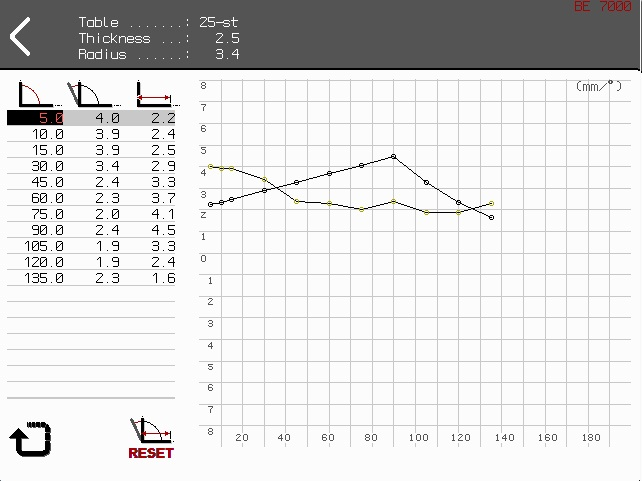
\includegraphics[width=0.8\textwidth, clip]{appA/images/schwenkbiegen_1}
    \end{tcolorbox}
    \caption{Example of an technology table.}
    \label{fig:technology-table}
\end{figure}

\section{Hyper Parameters}\label{sec:hyper-parameters}

The following sections show all the hyper-parameters used to train the \ac{ML} models of this study.
They can be also found in the source code accompanying this thesis.

\subsection{Decision Tree}
Grid search cross validation was used to find the best hyper-parameters for
the decision tree.
All hyper-parameters are summarized in Table~\ref{tab:hyperparameters_decision_tree}.

\begin{table}[H]
    \begin{tcolorbox}[arc=0pt,boxrule=0.5pt]
        \sisetup{group-minimum-digits = 4}
        \centering
        \begin{tabular}{ll}
            \toprule
            \thead{\textbf{Hyperparameter}} & \thead{\textbf{Value}} &
            \thead{\textbf{Description}}
            \\
            \toprule
            criterion & absolute\_error
            \hdashline
            max\_depth & 30 \\
            \hdashline
            min\_samples\_split & 4 \\
            \hdashline
            min\_weight\_fraction\_leaf & 0. \\
            \hdashline
            splitter & random \\
            \hdashline
            ccp_alpha & 0.0 \\
            \bottomrule
        \end{tabular}
        \caption{Hyperparameters of \ac{DT} model.}
        \label{tab:hyperparameters_decision_tree}
    \end{tcolorbox}
\end{table}

\subsection{Random Forest}

\begin{table}[H]
    \begin{tcolorbox}[arc=0pt,boxrule=0.5pt]
        \sisetup{group-minimum-digits = 4}
        \centering
        \begin{tabular}{ll}
            \toprule
            \thead{\textbf{Hyperparameter}} & \thead{\textbf{Value}} &
            \thead{\textbf{Description}}
            \\
            %  \unit{(Kcal\per\mole)\squared}}} & \thead{RMSD l.b.} &
            %  \thead{RMSD u.b.}  \\
            \toprule
            n\_estimators & 10 & The number of trees in the forest.
            \\
            \hdashline
            criterion & absolute\_error \\
            \hdashline
            max\_depth & 30 \\
            \hdashline
            min\_samples\_split & 4 \\
            \hdashline
            min\_samples\_leaf & 2 \\
            \hdashline
            max\_features & auto \\
            \hdashline
            max\_leaf\_nodes & X \\
            \hdashline
            max\_leaf\_nodes & X \\
            \bottomrule
        \end{tabular}
        \caption{Hyperparameters of the \ac{RF} model.}
        \label{tab:hyperparameters_rf}
    \end{tcolorbox}
\end{table}

\subsection{Extra Trees}

\begin{table}[H]
    \begin{tcolorbox}[arc=0pt,boxrule=0.5pt]
        \sisetup{group-minimum-digits = 4}
        \centering
        \begin{tabular}{ll}
            \toprule
            \thead{\textbf{Hyperparameter}} & \thead{\textbf{Value}} &
            \thead{\textbf{Description}}
            \\
            %  \unit{(Kcal\per\mole)\squared}}} & \thead{RMSD l.b.} &
            %  \thead{RMSD u.b.}  \\
            \toprule
            bootstrap & True
            \\
            \hdashline
            criterion & absolute\_error \\
            \hdashline
            max\_depth & 6 \\
            \hdashline
            min\_samples\_split & 4 \\
            \hdashline
            min\_samples\_leaf & 1 \\
            \bottomrule
        \end{tabular}
        \caption{Hyperparameters of the Extra Trees model.}
        \label{tab:hyperparameters_et}
    \end{tcolorbox}
\end{table}

\subsection{Gradient Boosting}

\begin{table}[H]
    \begin{tcolorbox}[arc=0pt,boxrule=0.5pt]
        \sisetup{group-minimum-digits = 4}
        \centering
        \begin{tabular}{ll}
            \toprule
            \thead{\textbf{Hyperparameter}} & \thead{\textbf{Value}} &
            \thead{\textbf{Description}}
            \\
            \toprule
            loss & huber
            \\
            \hdashline
            learning\_reate & 0.1 \\
            \hdashline
            max\_depth & 4 \\
            \hdashline
            min\_samples\_split & 3 \\
            \hdashline
            min\_samples\_leaf & 3 \\
            \hdashline
            n\_estimators & 200 \\
            \bottomrule
        \end{tabular}
        \caption{Hyperparameters of the Extra Trees model.}
        \label{tab:hyperparameters_gradient_boosting}
    \end{tcolorbox}
\end{table}

\subsection{SVM}

\begin{table}[H]
    \begin{tcolorbox}[arc=0pt,boxrule=0.5pt]
        \sisetup{group-minimum-digits = 4}
        \centering
        \begin{tabular}{ll}
            \toprule
            \thead{\textbf{Hyperparameter}} & \thead{\textbf{Value}} &
            \thead{\textbf{Description}}
            \\
            \toprule
            bootstrap & True \\
            \hdashline
            criterion & absolute\_error \\
            \hdashline
            min\_samples\_split & 4 \\
            \hdashline
            max\_depth & 6 \\
            \hdashline
            min\_samples\_leaf & 1 \\
            \hdashline
            n\_estimators & 10 \\
            \bottomrule
        \end{tabular}
        \caption{Hyper-paramters of the SVM model.}
        \label{tab:hyperparameters_svm}
    \end{tcolorbox}
\end{table}

\subsection{MLP}

\begin{table}[H]
    \begin{tcolorbox}[arc=0pt,boxrule=0.5pt]
        \sisetup{group-minimum-digits = 4}
        \centering
        \begin{tabular}{ll}
            \toprule
            \thead{\textbf{Hyperparameter}} & \thead{\textbf{Value}} &
            \thead{\textbf{Description}}
            \\
            %  \unit{(Kcal\per\mole)\squared}}} & \thead{RMSD l.b.} &
            %  \thead{RMSD u.b.}  \\
            \toprule
            random\_state & 1 \\
            \hdashline
            solver & lbfgs \\
            \hdashline
            max\_iter & 5000 \\
            \hdashline
            alpha & 0.01 \\
            \hdashline
            hidden\_layer\_sizes & (100, 100) \\
            \hdashline
            learning\_rate & constant \\
            \bottomrule
        \end{tabular}
        \caption{Hyperparameters of the \ac{MLP} model.}
        \label{tab:hyperparameters_mlp}
    \end{tcolorbox}
\end{table}
